\chapter{Komunikační modul Wireless M-Bus}
\label{ChapterKomunikacniModul}

Spolu se zařízením UniPi Neuron S103 byl zapůjčen i modul IQRF TR-72DC-WMB, který do budoucna bude součástí tohoto produktu a bude rozšiřovat konektivitu zařízení o protokol Wireless M-Bus. 

\section{Obecný popis modulu TR-72D-WMB}

Modul IQRF TR-72DA-WMB je bezdrátový komunikační modul velikosti SIM karty z výroby české firmy \href{http://microrisc.com/cs/}{MICRORISC s.r.o.}. Vychází z řady produktů technologie IQRF, s tím rozdílem, že místo IQRF softwaru má přímo implementovaný Wireless M-Bus protokol \cite{ModulIQRF}. 

 \begin{figure}[!ht]
\vspace{-1,pt}
  \begin{center}
    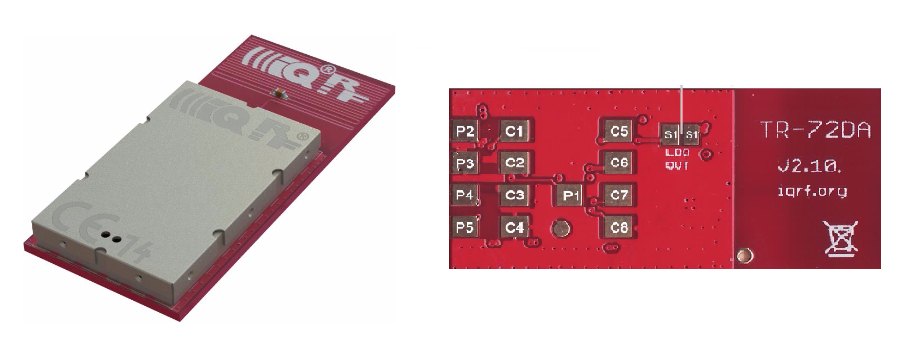
\includegraphics[scale=0.76]{obrazky/modul_modul}
  \end{center}
	\vspace{-20pt}
  \caption{Modul IQRF TR-72DA-WMB \cite{ModulIQRF}}
	\vspace{-10pt}
\end{figure}

Na malém prostoru se nachází vše potřebné pro uskutečnění bezdrátového přenosu: mikrokontrolér, externí EEPROM, teplotní senzor, kontrolní LED, 6 pinů a~anténa dle typu komunikačního modulu (Obr.~\ref{BlokovkaIQRF}).



Modul podporuje módy přenosu S1, S2, T1 a T2. Napájecí napětí modulu je~v~rozsahu 3,1 až 5,3\,V se spotřebou 1\,$\mu$A v režimu spánku a 8-22\,mA ve vysílacím režimu, dle nastavení výstupního výkonu, jehož maximální hodnota je 12,5\,W.
V~České republice je využíván pro přenos v bezlicenčním pásmu 868\,MHz, případně 433\,MHz nebo 169\,MHz.\newline

\newpage

 \begin{figure}[!ht]
	\vspace{-20pt}
  \begin{center}
    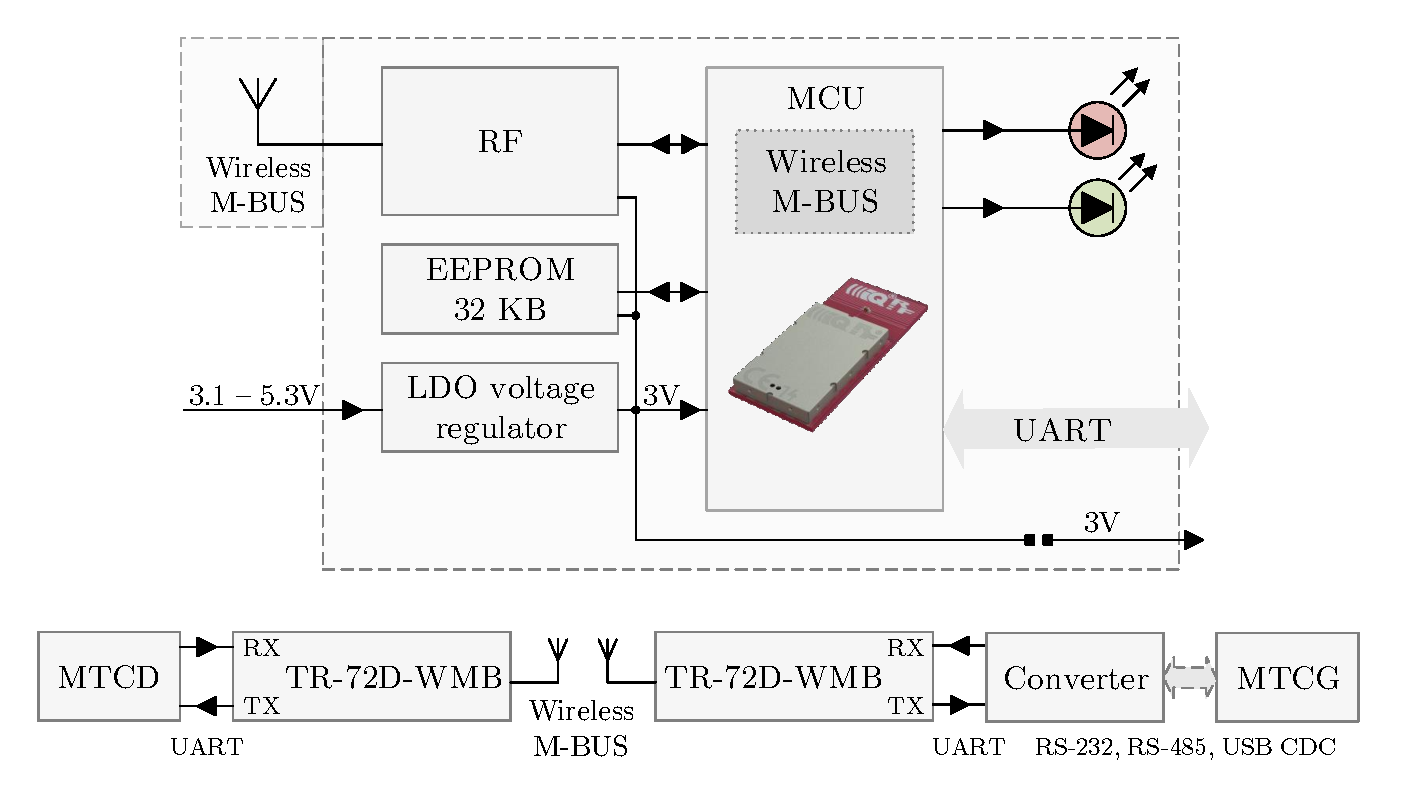
\includegraphics[scale=0.6]{obrazky/modul_block}
  \end{center}
	\vspace{-30pt}
  \caption{Blokové schéma modulu TR-72D-WMB \cite{ModulIQRF}}
	\label{BlokovkaIQRF}
	\vspace{-5pt}
\end{figure}

Modul je vyráběn ve třech verzích (viz Obr.~\ref{ObrazekAnteny}) dle připojení antény:
\begin{itemize}
		\item TR-72D-WMB má zdířku pro připájení antény.
		\item TR-72DC-WMB	má vyveden koaxiální anténí konektor U.FL. 
		\item TR-72DA-WMB má integrovanou anténu přímo na desce modulu. Dosah signálu toto typu je až 320\,m v módu T a 365\,m v módu S.
\end{itemize}

\begin{figure*}[!ht]
    \centering
			\subfigure[TR-72D-WMB]{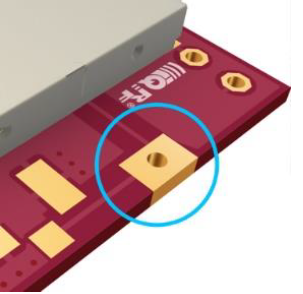
\includegraphics[width=0.28\textwidth]{obrazky/modul_antenaa}\label{modul_antenaa}}
			\hspace*{5mm}
			\subfigure[TR-72DC-WMB]{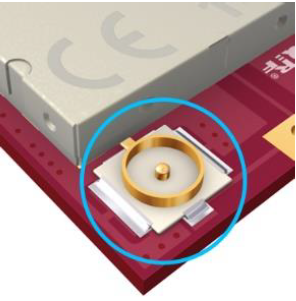
\includegraphics[width=0.28\textwidth]{obrazky/modul_antenab}\label{modul_antenab}}
			\hspace*{5mm}
			\subfigure[TR-72DA-WMB]{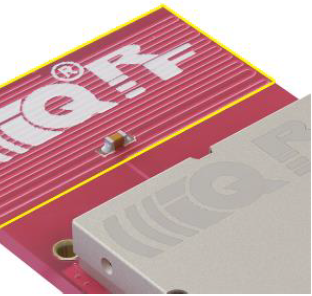
\includegraphics[width=0.28\textwidth]{obrazky/modul_antenac}\label{modul_antenac}}
		\caption{Přehled typu modulu dle antény \cite{ModulIQRF}}
		\label{ObrazekAnteny}
		\vspace{-20pt}
\end{figure*}

\section{Komunikační módy}

Modul může být v závislosti na použité topologii nastaven do jednoho ze tří provozních módů: měřič, koncentrátor, skener \cite{ModulIQRF}. 

V módu měřiče může být modul přes UART sběrnici zapojen k mikrokontroléru, který zajistí zpracování dat od senzorů. Může tedy sloužit k sestavení vlastních měřicích zařízení postavených na protokolu Wireless M-Bus.

V módu koncentrátoru slouží modul jako komunikační zařízení pro sběr dat z~meřičů. Aktuální firmware podporuje pouze obousměrnou komunikaci s měřiči v~režimu S a T a je zatím ve fázi vývoje a do produkce nasazen jako experimentální. Z tohoto důvodu bude při implementaci samotné aplikace modul nasazen v režimu skeneru.

V módu skeneru modul zachytává veškerou dostupnou komunikaci daného módu přenosu. Díky vnitřní implementaci Wireless M-Bus protokolu je modul schopen zachytávat a dešifrovat šifrovanou komunikaci, je však nutné počítat s tím, že současný firmware není stavěný na vyžití modulu pro příjem šifrované komunikace v módu skeneru od více zařízení zároveň. Modul totiž automaticky veškeré zachycené šifrované telegramy automaticky rozšifruje pomocí jediného interního AES klíče. Jedná se však o klíč daného modulu, nikoliv vyčítaného zařízení. Při vyčítání šifrovaných dat je tedy nutné postupovat složitěji a provést nejdříve zpětné zašifrování daných dat tímto klíčem a až poté provést rozšifrování dat dle normy.

Praktické využíti jednotlivých módu zobrazuje Obr.~\ref{TopologieIQRF}.

 \begin{figure}[!ht]
\vspace{-20pt}
  \begin{center}
    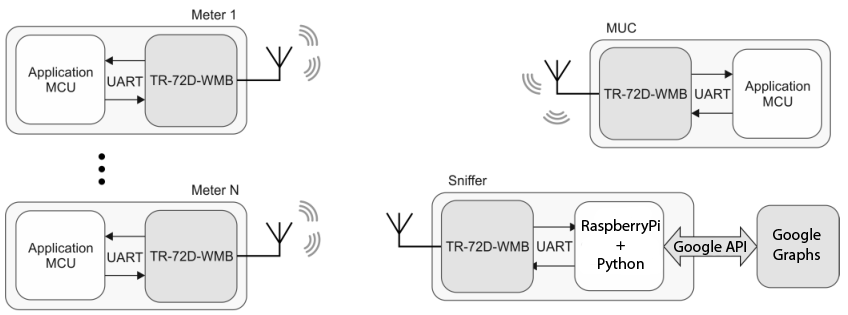
\includegraphics[scale=0.65]{obrazky/modul_topologie}
  \end{center}
	\vspace{-30pt}
  \caption{Různé módy dle použité topologie \cite{ModulIQRF}}
	\label{TopologieIQRF}
	\vspace{-20pt}
\end{figure}

\section{Komunikační protokol}

S řídícím mikrokontrolérem modul komunikuje pomocí rozhraní UART, jehož parametry jsou 19200\,Bd, 8\,bitů, žádná parita a 1 stop bit.
		
Modul podporuje jednoduchý formát příkazů sloužící k nastavení konfiguračních parametrů modulu i k samotné komunikaci s modulem. Každý příkaz začíná znakem \texttt{\textgreater}. Každá zpráva odpověďi začíná znakem \texttt{\textless}. Každému příkazu musí předcházet budící znak \texttt{NULL (0x00)} následovaný 2\,ms pauzou a každý paket příkazů je ukončen znakem \texttt{CR (0x0D)}. 

\newpage
Obecná struktura~\cite{ModulIQRF}~paketu příkazu je 

\begin{figure}[!ht]
\begin{centerverbatim}
			>[CC][RW][DATA][CR]
\end{centerverbatim}
\end{figure}

kde CC je jednobajtový kód daného příkazu, RW je jednobajtový příznak zápisu (\textbf{:}) či čtení dat (\textbf{?}) dat, DATA jsou zapisovaná data, pokud se jedná o zápis a CR je znak ukončení.

Obecná skruktura odpovědi je následující

\begin{figure}[!ht]
\begin{centerverbatim}
	<[DATA][CR]
\end{centerverbatim}
\end{figure}

kde DATA obsahuje přenášená data či návratové kódy (OK pro správné dokončení příkazu, ERR1 pro chybu syntaxe a ERR2 pro neplatnou vstupní hodnotu). Některé bajty jsou kódovány v šestnáckové soustavě či využívají uložení BigEndian.

Například dotaz a odpověd pro aktuální AES klíč je:
\label{KapitolaStazeniKlice}

\begin{figure}[!ht]
\begin{centerverbatim}
	>03?[CR]
	<010203040506070809a0b0c0d0e0f[CR]  
\end{centerverbatim}
\end{figure}

a pro případnou změnu AES klíče:

\begin{figure}[!ht]
\begin{centerverbatim}
>03:112233445566778899aabbccddeeff[CR]
>OK[CR]
\end{centerverbatim}
\end{figure}

Ukázku jednoduché komunikace s modulem v jazyce Python obsahuje~Kód~\ref{CodeSerial}.

\begin{lstlisting}[caption={Komunikace s modulem přes sériový port},captionpos=b,label=CodeSerial,style=MyCodePython]
import serial

# Setup a serial port
	ser = serial.Serial(
		port='/dev/ttyAMA0',
		baudrate=19200,
		parity=serial.PARITY_NONE,
		stopbits=serial.STOPBITS_ONE,
		bytesize=serial.EIGHTBITS,
		timeout=1
	)
  output("SCR", "Device is ready: " + str(ser.isOpen()))

# Set default AES key
	ser.write("\x00\x00>03:" + AES_IQRF_DEFAULT + "\x0D")
	y = ser.readline()
	output("SCR", "Default AES key set: " + y[1:])
\end{lstlisting}



